\documentclass[12pt]{article}
\usepackage{graphicx}
\usepackage{geometry}
\usepackage{listings}
\geometry{a4paper, margin=1in}

\title{Lab Task with Command Summary}
\author{Muhammad Shafeen \\ 22P-9278 \\ BS AI}
\date{}

\begin{document}

\maketitle

\section*{Introduction}
This document contains a summary of Linux commands executed during the lab task. Each section includes a screenshot of the command and its description, along with the commands and their respective outputs.

\section*{Image Descriptions and Commands}

\subsection*{Image 1}
\begin{figure}[h!]
    \centering
    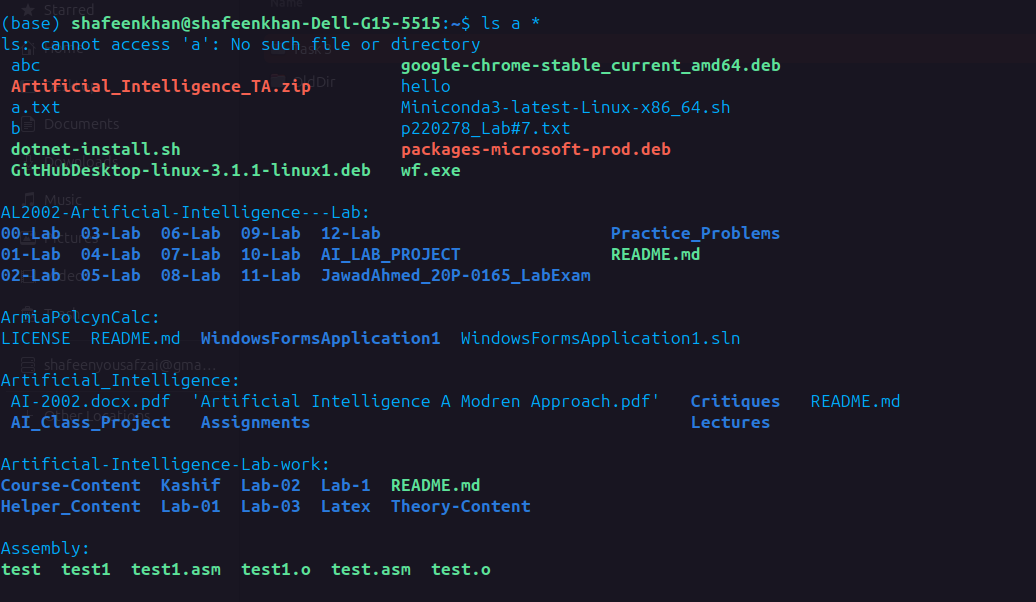
\includegraphics[width=0.5\textwidth]{1.png}
    \caption{Removing files and using `cat` command to create and append content to a file.}
\end{figure}
\begin{lstlisting}
rm newfile
cat > hello.txt
cat hello.txt
cat >> hello.txt
cat hello.txt
\end{lstlisting}
- Description: In this sequence, the `rm` command deletes `newfile`. The `cat >` command creates `hello.txt` with content, and `cat >>` appends more text. The file's contents are displayed using `cat hello.txt`.

\subsection*{Image 2}
\begin{figure}[h!]
    \centering
    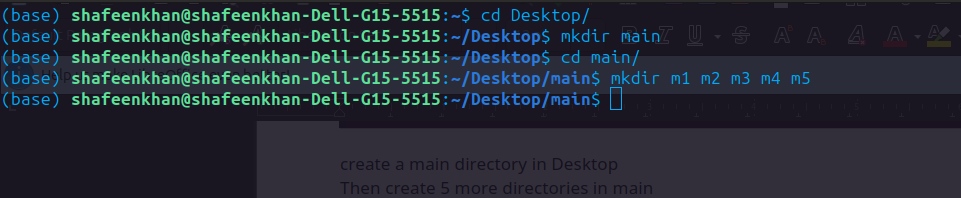
\includegraphics[width=0.5\textwidth]{2.png}
    \caption{Removing a file using the `rm` command.}
\end{figure}
\begin{lstlisting}
rm newfile
\end{lstlisting}
- Description: The `rm` command deletes the file `newfile`.

\subsection*{Image 3}
\begin{figure}[h!]
    \centering
    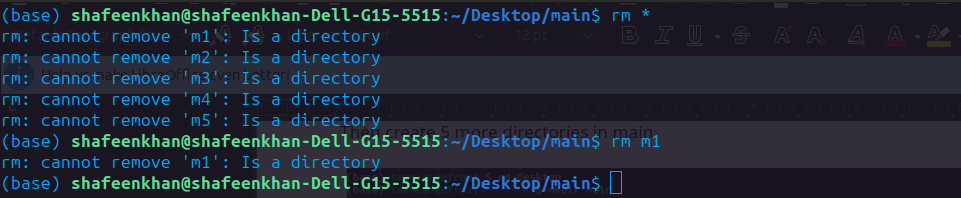
\includegraphics[width=0.5\textwidth]{3.png}
    \caption{Redirecting the output of `ls` to a new file.}
\end{figure}
\begin{lstlisting}
ls > newfile
cat < newfile
\end{lstlisting}
- Description: The `ls` command output is redirected to `newfile`, and the content of `newfile` is displayed using `cat`.

\subsection*{Image 4}
\begin{figure}[h!]
    \centering
    
\includegraphics[width=0.5\textwidth]{4.png}
    \caption{Creating a new file using `touch`.}
\end{figure}
\begin{lstlisting}
touch newfile3
ls
\end{lstlisting}
- Description: The `touch` command is used to create an empty file called `newfile3`, and the directory contents are listed using `ls`.

\subsection*{Image 5}
\begin{figure}[h!]
    \centering
    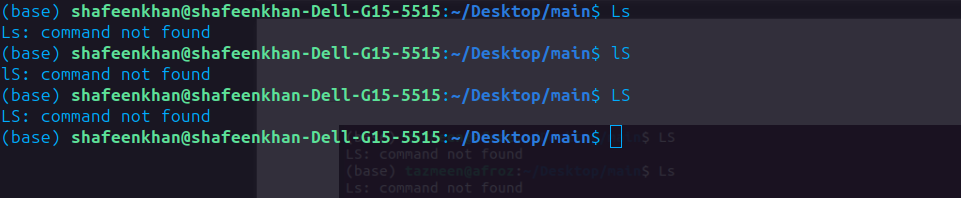
\includegraphics[width=0.5\textwidth]{5.png}
    \caption{Changing directory and listing contents.}
\end{figure}
\begin{lstlisting}
cd textfiles
ls
\end{lstlisting}
- Description: The `cd` command navigates to the `textfiles` directory, and `ls` lists its contents.

\subsection*{Image 6}
\begin{figure}[h!]
    \centering
    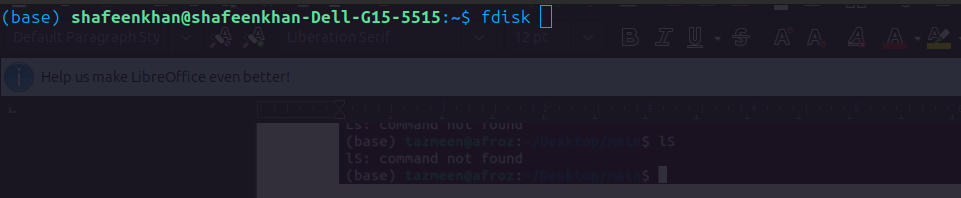
\includegraphics[width=0.5\textwidth]{6.png}
    \caption{Copying content from one file to another.}
\end{figure}
\begin{lstlisting}
cat a.txt > b.txt
nano b.txt
cat b.txt
\end{lstlisting}
- Description: The content of `a.txt` is copied to `b.txt` using `cat >`. The `nano` command opens `b.txt` for editing, and `cat b.txt` displays its content.

\subsection*{Image 7}
\begin{figure}[h!]
    \centering
    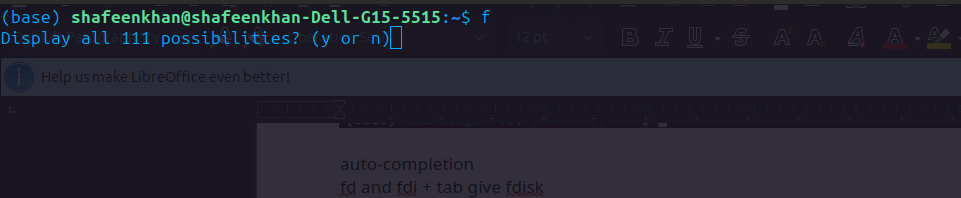
\includegraphics[width=0.5\textwidth]{7.png}
    \caption{Displaying a file's content with line numbers.}
\end{figure}
\begin{lstlisting}
cat -n a.txt
\end{lstlisting}
- Description: The `cat -n` command displays the content of `a.txt` with line numbers.

\subsection*{Image 8}
\begin{figure}[h!]
    \centering
    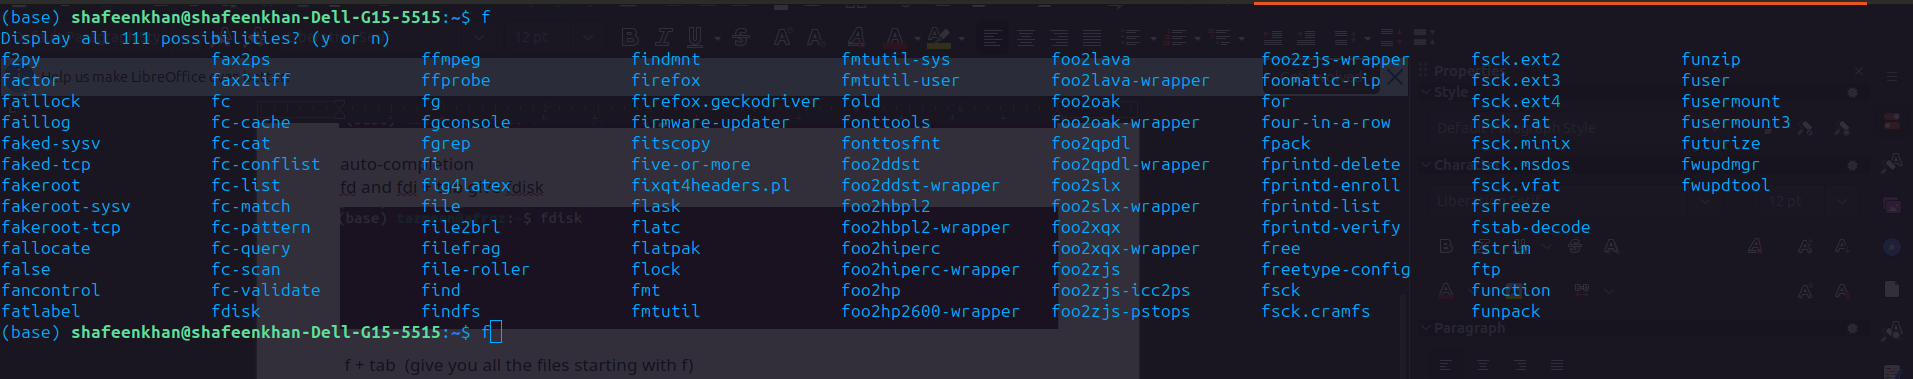
\includegraphics[width=0.5\textwidth]{8.png}
    \caption{Displaying the content of two files.}
\end{figure}
\begin{lstlisting}
cat a.txt b.txt
\end{lstlisting}
- Description: The `cat` command displays the combined content of `a.txt` and `b.txt`.

\subsection*{Image 9}
\begin{figure}[h!]
    \centering
    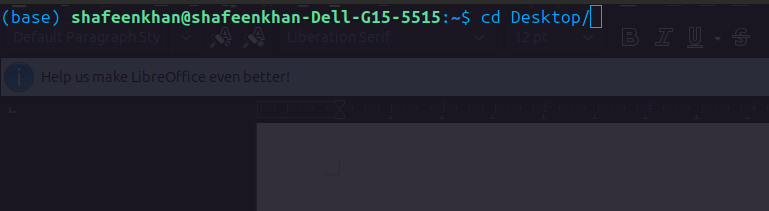
\includegraphics[width=0.5\textwidth]{9.png}
    \caption{Using `echo` to write to a file.}
\end{figure}
\begin{lstlisting}
echo Hello World
cat a.txt
\end{lstlisting}
- Description: The `echo` command writes "Hello World" to the terminal, and `cat a.txt` displays the content of `a.txt`.

% Continue for remaining images
\subsection*{Image 10}
\begin{figure}[h!]
    \centering
    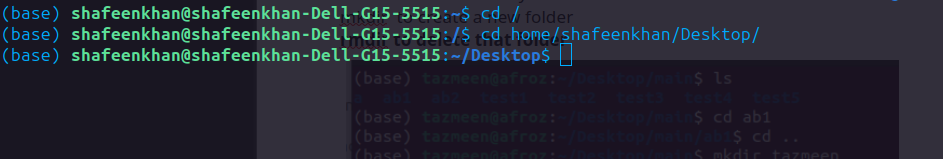
\includegraphics[width=0.5\textwidth]{10.png}4
    \caption{Displaying content of a file and counting lines using `cat -n`.}
\end{figure}
\begin{lstlisting}
cat -n file.txt
\end{lstlisting}
- Description: The `cat -n` command displays the content of `file.txt` with line numbers.

\subsection*{Image 11}
\begin{figure}[h!]
    \centering
    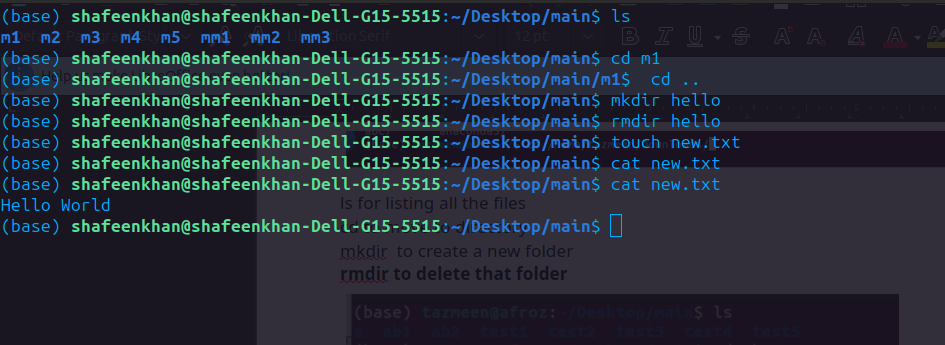
\includegraphics[width=0.5\textwidth]{11.png}
    \caption{Removing a directory using `rm -r`.}
\end{figure}
\begin{lstlisting}
rm -r dir1


\end{lstlisting}
- Description: The `rm -r` command removes the directory `dir1` and its contents recursively.

\subsection*{Image 12}
\begin{figure}[h!]
    \centering
    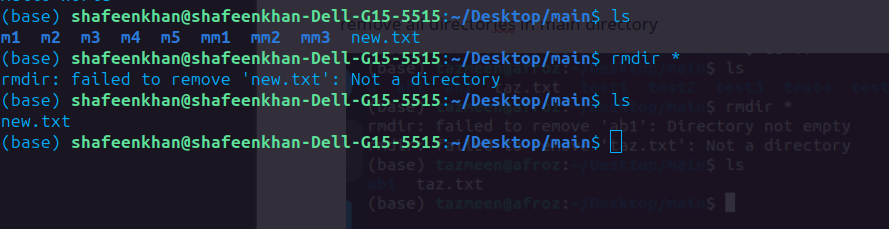
\includegraphics[width=0.5\textwidth]{12.png}
    \caption{Appending text to a file using `cat >>`.}
\end{figure}
\begin{lstlisting}
cat >> file.txt
\end{lstlisting}
- Description: The `cat >>` command appends content to `file.txt`.

\subsection*{Image 13}
\begin{figure}[h!]
    \centering
    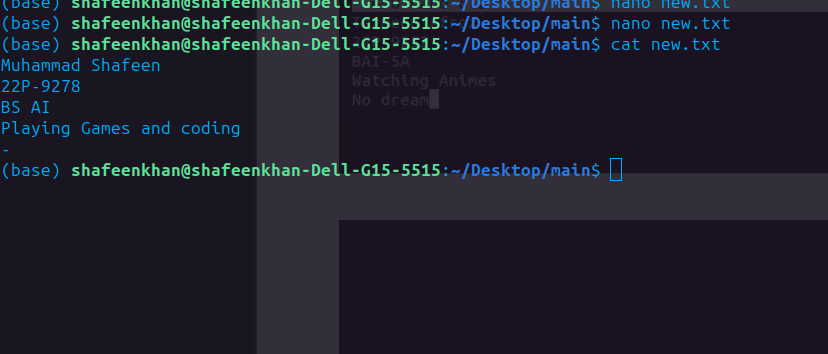
\includegraphics[width=0.5\textwidth]{13.png}
    \caption{Creating nested directories using `mkdir -p`.}
\end{figure}
\begin{lstlisting}
mkdir -p dir1/dir2/dir3
\end{lstlisting}
- Description: The `mkdir -p` command creates nested directories `dir1/dir2/dir3`.

\subsection*{Image 14}
\begin{figure}[h!]
    \centering
    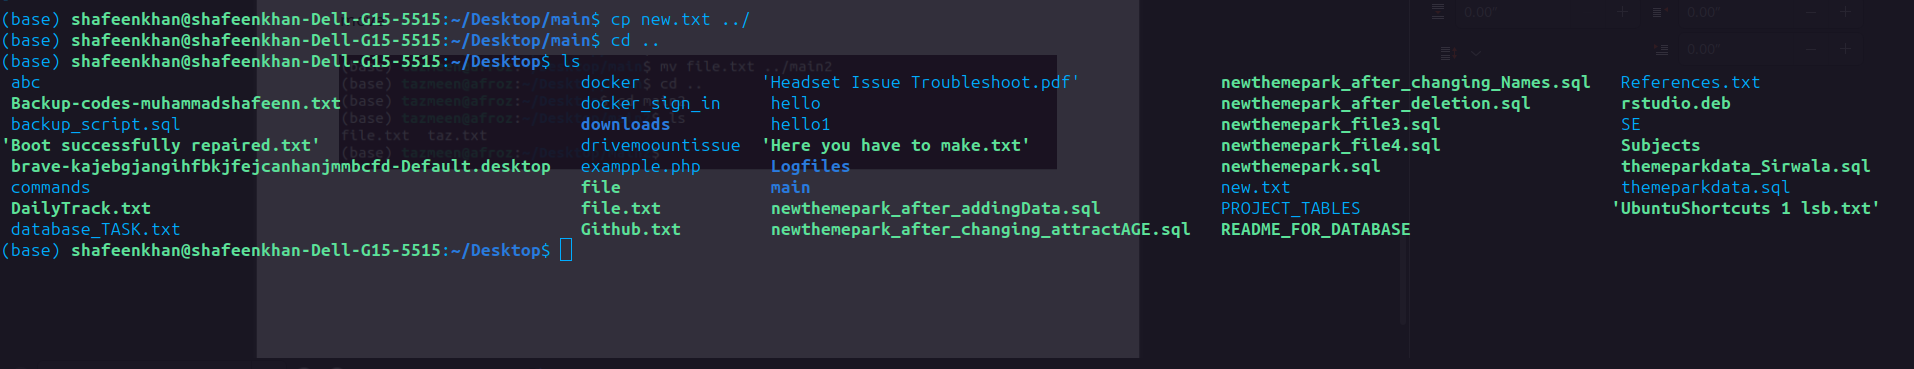
\includegraphics[width=0.5\textwidth]{14.png}
    \caption{Displaying directory contents recursively using `ls -R`.}
\end{figure}
\begin{lstlisting}
ls -R
\end{lstlisting}
- Description: The `ls -R` command lists the contents of directories and subdirectories recursively.

\subsection*{Image 15}
\begin{figure}[h!]
    \centering
    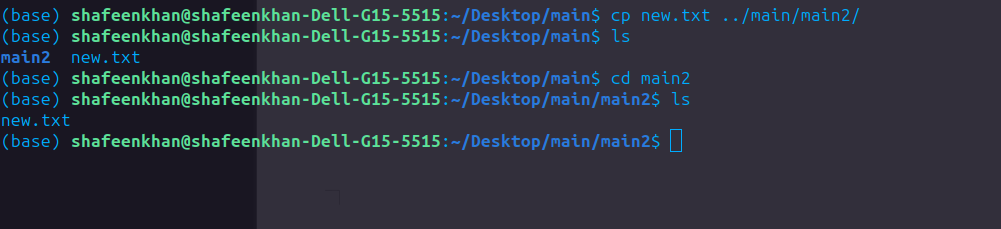
\includegraphics[width=0.5\textwidth]{15.png}
    \caption{Removing a directory and its contents using `rm -rv`.}
\end{figure}
\begin{lstlisting}
rm -rv dir1
\end{lstlisting}
- Description: The `rm -rv` command removes `dir1` and its contents, showing verbose output.

\subsection*{Image 16}
\begin{figure}[h!]
    \centering
    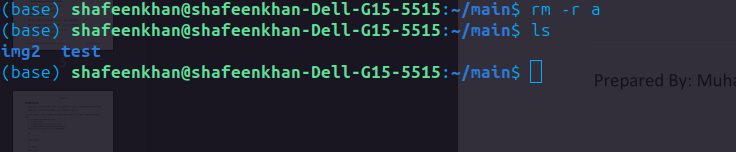
\includegraphics[width=0.5\textwidth]{16.png}
    \caption{Copying files using `cp`.}
\end{figure}
\begin{lstlisting}
cp file1.txt dir1/
\end{lstlisting}
- Description: The `cp` command copies `file1.txt` into the directory `dir1`.

\subsection*{Image 17}
\begin{figure}[h!]
    \centering
    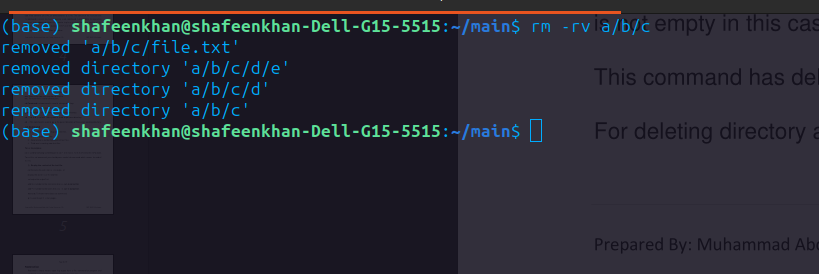
\includegraphics[width=0.5\textwidth]{17.png}
    \caption{Changing directory using `cd`.}
\end{figure}
\begin{lstlisting}
cd dir1
\end{lstlisting}
- Description: The `cd` command changes the current directory to `dir1`.

\subsection*{Image 18}
\begin{figure}[h!]
    \centering
    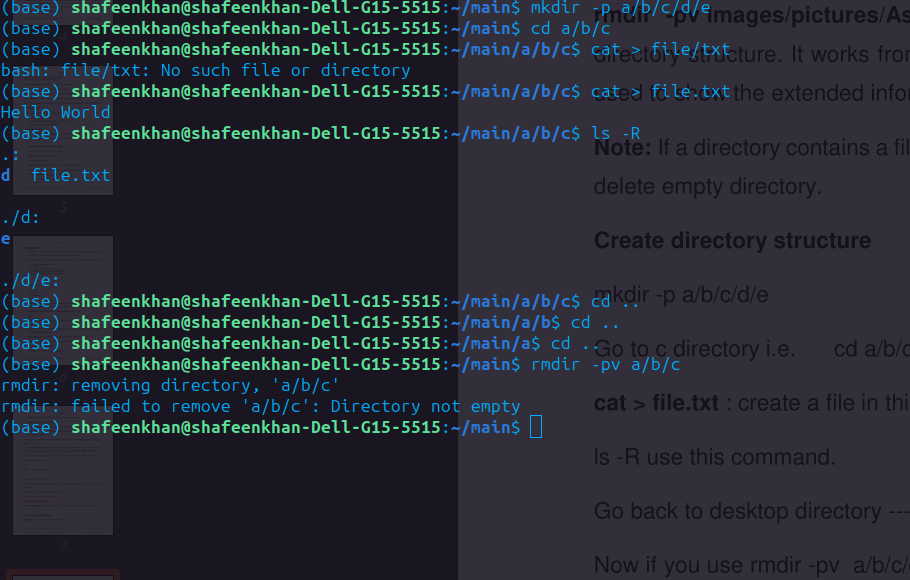
\includegraphics[width=0.5\textwidth]{18.png}
    \caption{Displaying file content using `cat`.}
\end{figure}
\begin{lstlisting}
cat file.txt
\end{lstlisting}
- Description: The `cat` command displays the content of `file.txt`.

\subsection*{Image 19}
\begin{figure}[h!]
    \centering
    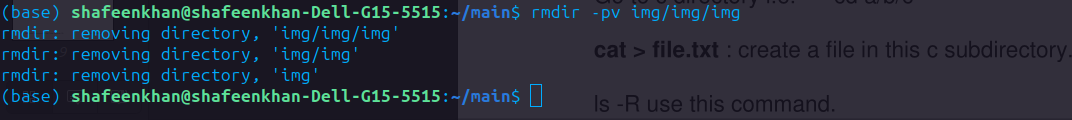
\includegraphics[width=0.5\textwidth]{19.png}
    \caption{Redirecting output using `>`.}
\end{figure}
\begin{lstlisting}
echo "Hello World" > file.txt
\end{lstlisting}
- Description: The `echo` command outputs "Hello World" into `file.txt`, overwriting any existing content.

\subsection*{Image 20}
\begin{figure}[h!]
    \centering
    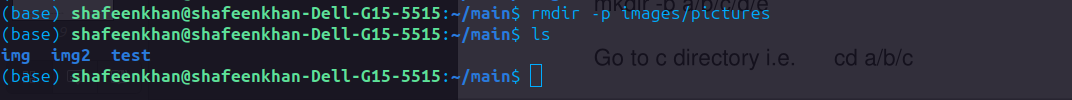
\includegraphics[width=0.5\textwidth]{20.png}
    \caption{Appending content to a file using `>>`.}
\end{figure}
\begin{lstlisting}
echo "More text" >> file.txt
\end{lstlisting}
- Description: The `echo` command appends "More text" to `file.txt`.
\section*{Conclusion}
This document covered a series of Linux commands that were executed during the lab session. Commands like `rm`, `cat`, `ls`, `touch`, `nano`, and `echo` were used to manipulate files and directories, showcasing how to manage content and files in a Linux environment.

\end{document}
